\chapter{Bref historique du français en 5 étapes
  clés}\label{chap:hist}

Tout d'abord il me semble important de souligner que je ne suis ni
historien, ni linguiste, ni prof de français. Par conséquent si vous
souhaitez plus d'exhaustivité sur ce sujet je vous recommande vivement
la série de vidéos présenté par le professeur au Collège de France
Claude Hagège disponible gratuitement sur
\href{https://youtu.be/fjAuHvOMXFE}{YouTube}. Je me base
essentiellement sur l'ouvrage remarquablement concis et précis
\href{https://www.amazon.fr/gp/product/2844100015/ref=as\_li\_tl?ie=UTF8\&camp=1642\&creative=6746\&creativeASIN=2844100015\&linkCode=as2\&tag=wwwbecomefree-21\&linkId=985f3a849fd44728e8480993cf2d5490}{français
  lycée} écrit par
\href{https://fr.wikipedia.org/wiki/Pierre_Brunel#Autres}{Pierre
  Brunel}.

\begin{quote}
  \'Elève à l'\'Ecole normale supérieure (1958), il est
  reçu premier à l'agrégation de lettres classiques en 1962, puis
  prépare deux thèses sur Paul Claudel, obtenant son doctorat d'\'Etat
  en 1970.
\end{quote}

Voilà pour une brève présentation de Monsieur Brunel qui fera office
de source principale pour ce que je présenterai dans ce chapitre. Si
vous souhaitez absolument un ouvrage de référence sur le sujet alors
je ne saurais que trop vous recommander l'ouvrage complet, rigoureux
et sérieux du linguiste français Alain Rey\footnote{Attention, il
  s'agit d'un ouvrage conséquent 672 pages rien que pour le tome1 et
  donc il y a aussi un tome~2 !} \href{https://www.amazon.fr/gp/product/2262033110/ref=as_li_tl?ie=UTF8&camp=1642&creative=6746&creativeASIN=2262033110&linkCode=as2&tag=wwwbecomefree-21&linkId=2be27c37e2162a822bb18af72db66042}{Mille ans de langue
  française tome 1}.\par

Et si vous vous intéressez en particulier à l'histoire de France alors
je vous recommande l'excellent ouvrage de Jean-Paul
Demoule\footnote{Vous pouvez déjà consulter son intervention dans
  une émission de Mediapart disponible sur \href{https://youtu.be/IMpHyq2gq7g?t=15m18s}{YouTube}.} \href{https://www.amazon.fr/gp/product/B00GNJHMUI/ref=as_li_tl?ie=UTF8&camp=1642&creative=6746&creativeASIN=B00GNJHMUI&linkCode=as2&tag=wwwbecomefree-21&linkId=d4b515d26f9ade9ea3e0759b397590a2}{On
  a retrouvé l'histoire de France}.\par

Bon après toutes ces recommandations de lectures textuelles ou
visuelles, passons à présent au vif du sujet.\par

Alors voici le plan en 5 étapes :

\begin{enumerate}
\item Les origines de la langue française
\item Du français au latin
\item L'unification de la langue
\item La fixation de l'orthographe
\item La fixation de la grammaire
\end{enumerate}

Bien entendu, si vous êtes fâché avec l'histoire, ou si vous voulez
uniquement acquérir une compétence technique, ou si vous n'avez pas le
temps vous pouvez directement passer au chapitre n\no~\ref{chap:voy} page~\pageref{chap:voy}. En revanche,
dans tous les cas je vous recommande d'étudier la phonétique française
\underline{avant} celle de l'anglais.

\newpage
\minitoc
\newpage
\section{Les origines de la langue française}\label{sec:orgfr}

\begin{quote}
  Le français est au croisement du latin et du germain, l'ancien
  allemand. Le fond celte -- gaulois -- est presque totalement oublié,
  sauf dans quelques noms de lieux.
\end{quote}

Dès le départ le ton est donné dans l'ouvrage de Pierre
Brunel\footnote{Il s'agit de l'introduction  de la partie du livre \href{https://www.amazon.fr/gp/product/2844100015/ref=as\_li\_tl?ie=UTF8\&camp=1642\&creative=6746\&creativeASIN=2844100015\&linkCode=as2\&tag=wwwbecomefree-21\&linkId=985f3a849fd44728e8480993cf2d5490}{français
  lycée} consacrée aux origines de la langue française.}. Bon, comme
annoncé plus haut, je ne suis ni historien, ni linguiste, ni prof de
français par conséquent je vais aller droit au but.\par

\subsection{Le fond latin}\label{subsec:lat}

Entre 58 et 52 avant notre ère la Gaule est conquise par les
Romains. Conséquence immédiate, le peuple de Gaule\footnote{Comme la
  plupart des autres régions dominées par l'empire romain\dots à part
  d'irréductible <<~grands-bretons~>> et autres écossais\dots mais
  c'est une autre histoire dont nous parlerons dans un prochain
  chapitre.} se met à parler le latin (par forcément par gaieté de
c{\oe}ur nous en conviendrons).\par

Laissez mijoter pendant deux siècles environ et voilà pourquoi lorsque
les barbares arrivent\dots ben les Gaulois parlent vraiment latin.

\subsection{Le fond germanique}\label{subsec:germ}

Les invasions germaniques au moment de la chute de Rome, en 410, sont
à l'origine d'une nouvelle transformation linguistique. Mais cette
fois-ci c'est l'envahisseur qui va adopter la langue locale et non
imposer la sienne. D'ailleurs il me semble avoir appris à l'école que
le commencement de la France serait le baptême de Clovis, rois des
Francs originaires de Saxe\footnote{Comment appelle-t-on les habitants
de la Saxe déjà ? Les Saxons ! C'est marrant c'est comme dans
anglo-saxon\dots élémentaire mon cher Watson !} en 496.\par
En résumé, après avoir été latinisés, les gaulois ont été germanisés
mais ont gardé le latin et la chrétienté comme héritage culturel
dominant.

\section{Du latin au français}\label{sec:lat2fr}

\begin{quote}
  Les Romains ont envahi la Gaule par le sud : les langues d'oc sont
  donc plus proches du latin que les langues d'oïl.
\end{quote}

La citation du livre de Pierre Brunel\footnote{Comme annoncé plus haut
je me base toujours sur le livre \href{https://www.amazon.fr/gp/product/2844100015/ref=as\_li\_tl?ie=UTF8\&camp=1642\&creative=6746\&creativeASIN=2844100015\&linkCode=as2\&tag=wwwbecomefree-21\&linkId=985f3a849fd44728e8480993cf2d5490}{français
  lycée} que je recommande chaleureusement pour plus de détails.} a le
mérite d'être claire, concise et limpide.

\subsection{Langue d'oc, langue d'oïl}\label{subsec:langOcOil}

\begin{quotation}
  Oc et oil sont les deux manières de dire oui, au sud et au nord de
  la Loire, qui figure la barrière symbolique entre les deux parties
  du territoire.\par
  Plus proches de la langue cultivée qu'est le latin, les langues d'oc
  -- qui donneront son nom à la région Languedoc -- correspondent
  également à une civilisation moins brutale que celle du Nord. [\dots]
\end{quotation}

Je précise que l'auteur n'a pas mis le tréma mais sur
\href{https://fr.wikipedia.org/wiki/Langue_d\%27o\%C3\%AFl}{Wikipédia}\footnote{Qui propose en plus la phonétique ce qui m'incite à
  leur faire plus confiance sur ce point particulier (prononciation :
  o-il [ɔ.il], ou-il [u.il], oui [wi], o-ille [ɔj]).}


\begin{subfigures}
  \label{fig:fig4a5}
  %
  \begin{figure}
    \centering
    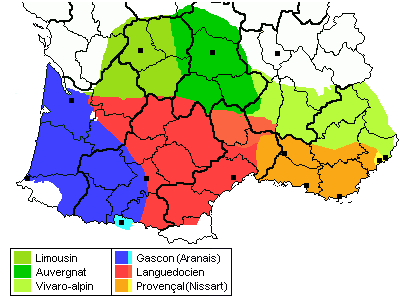
\includegraphics[scale=.725]{../img/langOc.png}
    \caption{Langue d'Oc}
    \label{fig:fig4}
  \end{figure}
  %
  \begin{figure}
    \centering
    \includegraphics[scale=.0725]{../img/langOil.png}
    \caption{Langue d'Oïl}
    \label{fig:fig5}
  \end{figure}
  %
\end{subfigures}

\subsection{L'ancien français}\label{subsec:ancienfr}

\begin{quotation}
  C'est la langue parlée au nord de la Loire. Du latin, elle garde
  l'essentiel de son vocabulaire, transformé par les prononciations
  locales, ainsi qu'une petite partie de sa grammaire, simplifiée :
  l'ancien français a encore une déclinaison, mais à deux cas
  seulement -- sujet et régime -- là ou le latin en comptait
  six. L'ordre des mots usuel\footnote{Vous trouverez facilement sur
    internet ou dans des ouvrages l'abréviation SVO pour \exFR{Sujet Verbe
    Objet} (\exEN{Subject Verb Object}).} -- sujet / verbe / complément -- est
  inédit : le latin s'exprimait dans l'ordre sujet / complément / verbe.
\end{quotation}

Pierre Brunel a tout dit dans cette sous-section alors passons à la
suite.

\subsection{Langue savante, langue vivante}\label{subsec:lslv}

\begin{quotation}
  Le latin populaire évolue très vite parce qu'il est parlé, souvent
  mal\footnote{Exactement comme l'anglais aujourd'hui.}, dans tout
  l'Empire. Il est à l'origine de l'ensemble des langues romanes que
  nous connaissons aujourd'hui -- italien, espagnol, portugais,
  roumain -- ainsi que de l'essentiel du français.
  La tradition du latin écrit est perpétuée par les moines. Elle fixe
  rapidement une langue de culture opposée aux langues populaires qui
  ne s'écrivent que très tardivement.
\end{quotation}

Durant le Moyen Âge 80\% de la littérature européenne est écrite en
latin, véritable lingua franca des élites intellectuelles. C'est aussi
la langue des sciences (et ça le restera encore
longtemps\footnote{Pensez à Newton qui a écrit son ouvrage majeur
  Principia Mathematica en latin.}). C'est d'ailleurs l'\'Eglise qui
contrôle les universités en Europe.


\section{L'unification de la langue}\label{sec:unifr}

\begin{quote}
  Le français s'est imposé très lentement, non seulement dans l'usage
  littéraire, dominé par le latin, mais dans la vie de tous les jours,
  où règnaient les langues régionales.
\end{quote}

\subsection{Un royaume éclaté en provinces}\label{subsec:roysplit}

\begin{quotation}
  Le sud de la France qui n'est pas, au Moyen Âge, encore intégré au
  royaume, est déjà framenté en divers <<~pays~>> dont les langues,
  pour proches qu'elles soient, ne sont pas absolument semblables.
  Ainsi, l4auvergne parle une langue d'oc que comprennent mal les gens
  de Bordeaux ou de Toulon.
  Au nord, la situation se complique. Seuls l'Île-de-France,
  l'Orléanais, la Picardie, la Normandie et l'Artois parlent français,
  avec des variantes.
  La Bourgogne -- du nord de Lyon aux Ardennes et de la Champagne à
  l'Alsace -- est pour l'essentiel un territoire germanique.
  La Bretagne est le refuge des derniers Celtes.
  Aux langues se superposent, de plus, des <<~patois~>>, utilisés sur
  des aires géographique plus restreintes, qui sont pafois peu compréhensibles.
\end{quotation}

\subsection{Le triomphe du Nord}\label{subsec:trinord}

\begin{quote}
  La plus grande unité politique de la France du Nord, la volonté
  expansionniste des rois de France, le fait que le Sud soit dans
  l'aire d'expansion arabe -- ce qui l'enrichit mais aussi le menace
  -- tout se ligue pour imposer la langue d'oil.
  Mais il faut attendre le \textsc{\romannumeral 15}\up{e}~siècle pour
  que la domination politique devienne une domination culturelle.
\end{quote}

\subsection{La langue du roi}\label{subsec:langroy}
\begin{quotation}
  L'édit de Villers-Cotterêts\footnote{Certaines personnes remettent
    en cause son importance comme dans cette \href{https://youtu.be/x3TQkQO_XMc}{vidéo}}, promulgué par François
  {\scshape{\romannumeral 1}}\up{er} en 1539, impose l'usage de la langue
  française dans les tribunaux. Ceux-ci utilisaient jusqu'alors
  exclusivement le latin et leurs décisions étaient donc mal comprises
  par le peuple.
  L'installation définitive de la cour du roi en Île-de-France impose
  peu à peu l'usage de la langue française aux seigneurs qui entourent
  le souverain.
\end{quotation}

\section{La fixation de l'orthographe}\label{sec:orthofix}

\begin{quote}
  Longtemps, le français s'est écrit comme il se parlait; vice versa,
  toutes les lettres se prononçaient, comme en latin. La notion même
  d'orthographe n'existait pas.
\end{quote}

\subsection{L'anarchie médiévale}\label{subsec:arnar}

\begin{quotation}
  Au Moyen Âge, il y a autant d'orthographes que de scripteurs. Les
  scribes, surtout des moines, sont plus intéressés par l'esthétique
  de leurs manuscrits que par une <<~correction~>> dont l'idée même
  n'existe pas. Ils ajoutent parfois des lettres, transforment un i en
  y pour bénéficier d'une courbe élégante.
  Les aristocrates, qui peu à peu apprennent à écrire, se soucient peu
  d'orthographe. 
\end{quotation}

\subsection{Les réformateurs du \textsc{\romannumeral
    16}\up{e}~siècle}\label{subsec:ref}
\begin{quotation}
  Plusieurs grammairiens comme Robert Estienne veulent écrire le
  français comme on l'entend et proposent des réformes visant à
  simplifier la graphie.
  On invente les accents pour rendre compte de la prononciation. On
  tente de supprimer les lettres qui ne se prononcent pas -- par
  exemple certains s terminaux hérités de la déclinaison de l'ancien
  français et la plupart des lettres doubles.
  L'absence de dictionnaire et, surtout, le manque d'intérêt des
  dirigeants, rendent toute généralisation difficile, d'autant que
  certains réformateurs, des humanistes tentés par la Réforme,
  manquent d'appuis à la Cour.
\end{quotation}

\subsection{Le triomphe des latinisants}\label{subsec:trilat}

\begin{quotation}
  Du Bellay affirme que le français vaut bien le latin : toutefois,
  langue et culture latines restent exemplaires. On justifie donc
  l'orthographe par l'étymologie et on invente des séries de mots sur
  leur modèle latin. Ainsi, à partir de confidentia, qui avait évolué
  en confiance, on fabrique confidence.
\end{quotation}

\section{La fixation de la grammaire}\label{sec:fixgram}

\begin{quote}
  Largement tributaire du latin pour son vocabulaire, le français s'en
  dégage radicalement dans sa grammaire. Mais il n'a imposé ses
  différences que peu à peu.
\end{quote}

\subsection{La fin des déclinaisons}\label{subsec:findec}

\begin{quotation}
  Entre l'ancien français (\textsc{\romannumeral 9}\up{e} -
\textsc{\romannumeral 16}\up{e}~siècle) et le français moderne (à
partir du \textsc{\romannumeral 16}\up{e}~siècle), on distingue
souvent une période intermédiaire de <<~moyen français~>>
(\textsc{\romannumeral 15}\up{e}~siècle) durant laquelle se fixent les
caractères de la langue moderne -- en particulier, la disparition de
la déclinaison. L'ancien français avait deux cas, afin de distinguer
les sujets et les autres fonctions.
Dorénavant, seules subsistent les distinctions entre singulier et pluriel.
\end{quotation}

\subsection{L'ordre des mots de la phrase}\label{subsec:ordmot}

\begin{quotation}
  Le latin, surtout en poésie, pouvait se permettre un ordre des mots
  fantaisiste, puisque les déclinaisons indiquaient la fonction
  grammaticale. Il en est de même, de façon très atténuée, en ancien
  français. C'est la disparition des déclinaisons qui impose l'ordre
  régulier de la phrase de base -- sujet / verbe / complément --, que
  seuls les poètes oseront encore enfreindre. De même, la disparition
  de finales discriminantes impose l'usage généralisé de l'article,
  que le latin ignorait et que l'ancien français pratiquait modérément.
\end{quotation}

\subsection{Une langue épurée}\label{langpur}

\begin{quotation}
  Les poètes de la Pléiade manifestaient une grande liberté
  d'invention lexicale.
  Mais, dès le début du \textsc{\romannumeral 17}\up{e}~siècle,
  Malherbe reprend en main la grammaire et le lexique en fixant des
  bornes très étroites à l'innovation.
  Les mots d'origine provinciales sont bannis pour <<~gasconnisme~>>
  -- du nom de la province de Gascogne. On crée le terme éloquent de
  <<~barbarisme~>> -- <<~propre à la façon de parler des barbares~>>
  -- pour désigner tout mot peu conforme au <<~génie de la
  langue~>>. L'axe Rouen-Paris domine la vie intellectuelle de façon
  autoritaire. On épure la langue au nom du roi\dots pour mieux
  l'imposer au roi -- Henri \textsc{\romannumeral 4} est Gascon --
  ainsi qu'à son entourage, souvent composés d'<<~étrangers~>>. On
  interdira bientôt l'usage de tel ou tel terme décrété
  <<~mal-sonnant~>> ou <<~bas~>>. La langue littéraire ne vivra
  désormais plus que dans une atmosphère raréfiée.
\end{quotation}

\newpage
\minitoc
